\subsection{Administrative}
The Administrative use case represented in figure \ref{2img:[use]administrative} illustrate the several actions the actors may be involved to. In particular the ``Login'' case is shared by each entity and so it can be generalized for a non defined user that may acess the System.

The use cases are described following:
\begin{description}
\item[Login:] the actor authenticate himself in the System to retrieve the access permissions;
\item[Reporting:] Representative, Programmer and System manager have tasks that need to be logged in order to build a concrete and reliable System over the time and function, so each activity involved has to be registered in the Administration;
\item[Bureaucracy management:] is a facets cases where participate Representative, Business consultant, Secretary and Analyst, each one with different scope and functions.
\item[Sending order:] is the case which allow the Company to require materials from the supplier and is performed by the Secretary.
\item[Meeting management:] both Representative and Secretary are involved in this task in order to plan personal or virtual meeting either with an external entity or between internal personal.
\item[Project proposal:] once a task has been accepted the Project Manager should concentrate on its planning;
\item[Order prosposal:] the main objective is due the System Manager that is interested in the System hardware management; it describes the Company needs and send for approval.
\item[Maintenance schedule:] System Manager to mantain the System has to be supported in its tasks.
\end{description}


\begin{figure}
\begin{centering}
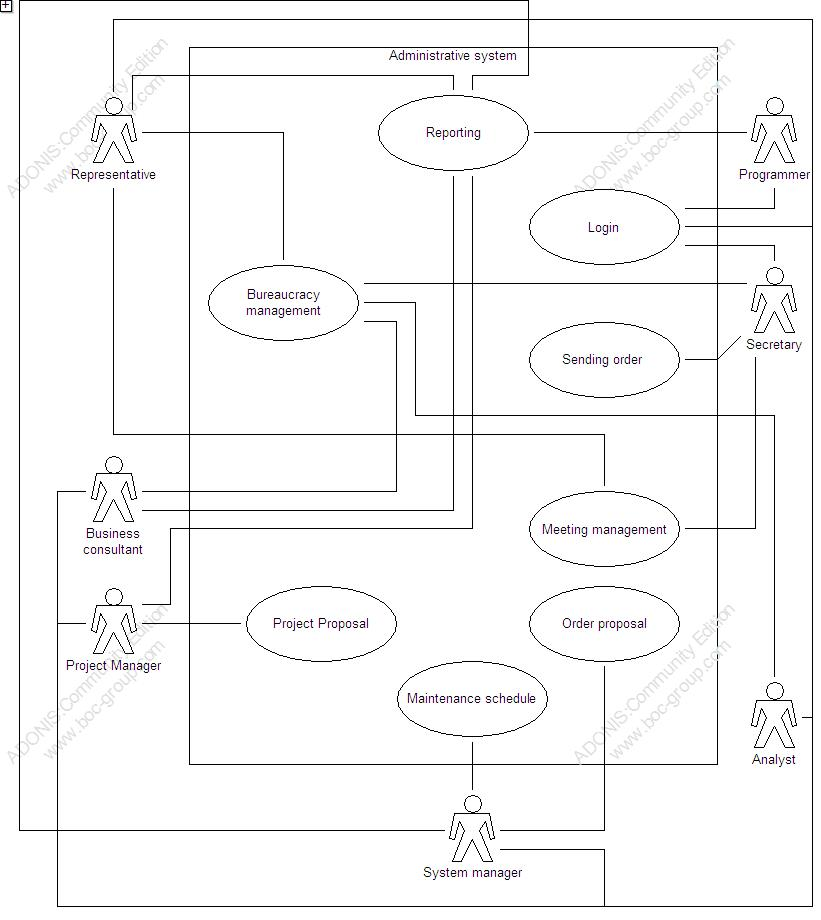
\includegraphics[scale=0.35]{assign3/adonis/imgs/administrative.jpg}
\caption{AllSpark Administrative use case.}
\label{2img:[use]administrative}
\end{centering}
\end{figure}


\subsection{Project}
The use case for Project, figured in \ref{2img:[use]project}, contains several interactions centered on the Project itself. In particular only three actors are involved in the work considering their objective.
The use cases are described following:
\begin{description}
\item[Status update:] allows the programmer to update its works status in order to mantain a guideline in the Project monitoring.
\item[Project planning:] supports both Project Manager and Analyst to perform the planning for a Project in all the several facets of the task.
\subitem[Team management:] allows to manage the team-mate, their objective, their reports with other team and so on;
\subitem[Team monitoring:] identify the behavior of the team during the project context.
\item[Checking work:] is a support case used in particular by the Analyst which has to observe the project status report since he has the knowledge to perform it, and in a second time also by the Project Manager for the proect conduct itself.
\item[Authorize resource instantiation:] sometimes is useful to manage the resources differently during the time and this is a supply for.
\end{description}

\begin{figure}
\begin{centering}
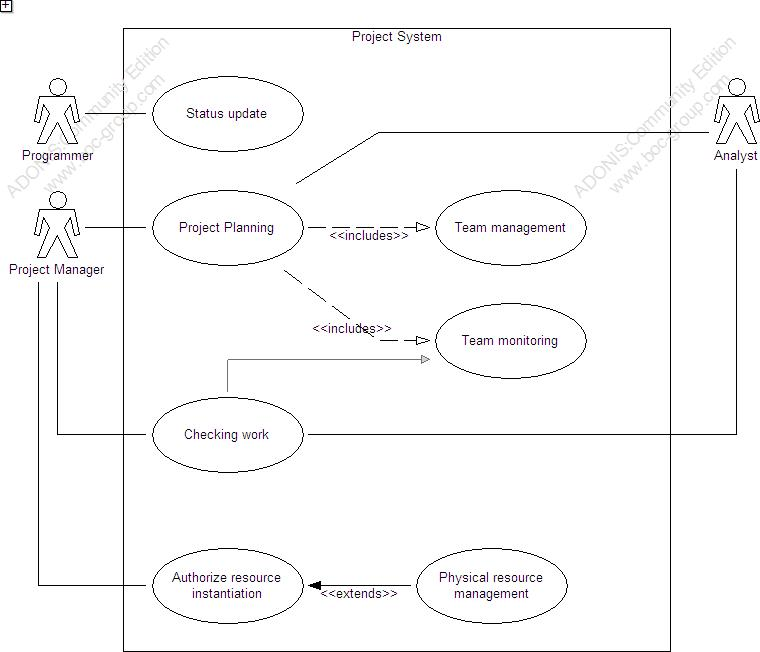
\includegraphics[scale=0.45]{assign3/adonis/imgs/project.jpg}
\caption{AllSpark Project use case.}
\label{2img:[use]project}
\end{centering}
\end{figure}

\subsection{Course}
The Course use case represented in \ref{2img:[use]Course} illustrates the several actions that the System should support in order to facilitate the entire management of a course. In particular the ``Lecturer'' is a generalization of several actors in that, depending on the course's subject, there may be requested specific skills.
\begin{description}
 \item[Course material Management:] is the supporting function aimed to easily manage the set of data provided by the Lecturer to student for a specified course.
 \item[Certification delivery:] once the student successful pass the examination owns the right to receive the certification of his studies that have to be confirmed by the Lecturer. The deliver of the acknoledgment has to be authorized by the Chief Executive Officier in that responsible of the Company granting the certificate.
 \item[Course logbook:] in order to mantaing a history about the course, this function support the Lecturer in the task of constantly track the program proposed.
 \item[Examination management:] once the students are ready, the examination process is performed to organize the validation sessions to achieve the certificate.
 \item[Timetable management:] planning a course is important to have a support in the not trivial management of the scheduled course during time.
\end{description}

\begin{figure}
\begin{centering}
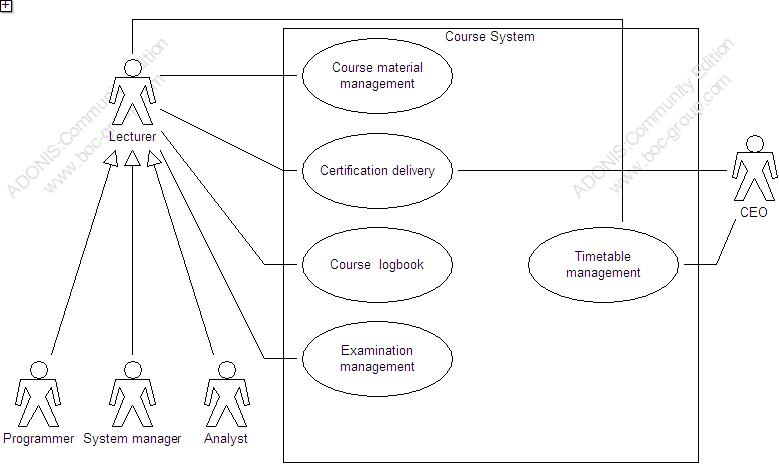
\includegraphics[scale=0.45]{assign3/adonis/imgs/course.jpg}
\caption{AllSpark Course use case.}
\label{2img:[use]Course}
\end{centering}
\end{figure}


\subsection{Commercial}
In order to support the Company in its decisions concerning the business finalities, the use case diagram illustrated in figure \ref{2img:[use]commercial} identify the main actions that actors may perform. In particular they are related on the customers' management and marketing campaign.
\begin{description}
 \item[Customers management:] is the important supply function that allow the Representative to mantain the contacts with the AllSpark's customer, in order to manage meeting, comunicate offers and general relationship affairs such as ``Product demos''.
 \item[Campaign planning:] is the Business operator objective to efficiently plan a marketing campaign and so different tools involve to support.
 \item[Manage Marketing campaign:] once the campaign has been planned the Secretary may monitor the trends of the campaign in order to present the result to Business operator.
\end{description}

\begin{figure}
\begin{centering}
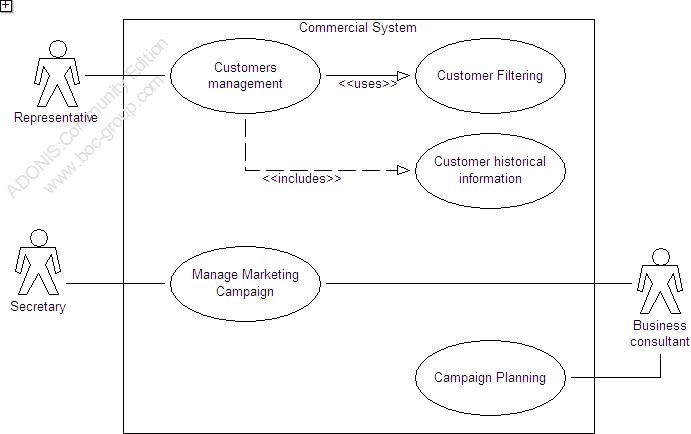
\includegraphics[scale=0.45]{assign3/adonis/imgs/commercial.jpg}
\caption{AllSpark Commercial use case.}
\label{2img:[use]commercial}
\end{centering}
\end{figure}


\subsection{Resource}
The real interesting resources that AllSpark need to manage are the system resources and this duty is entirely left to System Manager. The use case forseen represent the unique \textbf{inventory management} actions that supply the employee in the hardware inventory management. The systems used inside AllSpark are both software and hardware and the System Manager has to administrate both efficiently. The figure \ref{2img:[use]resource} illustrate the diagram just described.

\begin{figure}
\begin{centering}
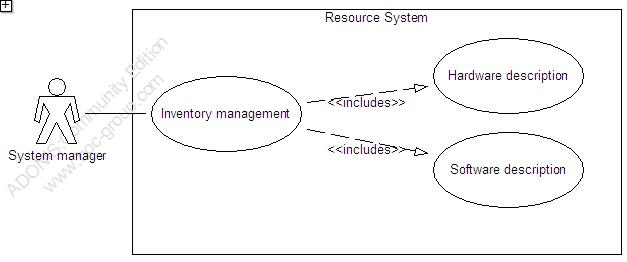
\includegraphics[scale=0.45]{assign3/adonis/imgs/resource.jpg}
\caption{AllSpark use case representing the Resource management.}
\label{2img:[use]resource}
\end{centering}
\end{figure}


\subsection{Documentation}
The issue in the Information Technology era is the massive presence of informations that may overfit each functions. The main idea of AllSpark is to efficiently manage the documentation concerning all kind of information regarding its products improving the search and presentation. The use case in figure \ref{2img:[use]documentation} shows the three actors involved in the production that use the \textbf{Editing documentation} function that aid the formatting and recording of all documentation related to a project. The Representative instead use a dedicated function\footnote{But it may be considered that the ``Editing documentation'' already implement a sort of kind.} to retrieve the essential informations that can interest the customer.

\begin{figure}
\begin{centering}
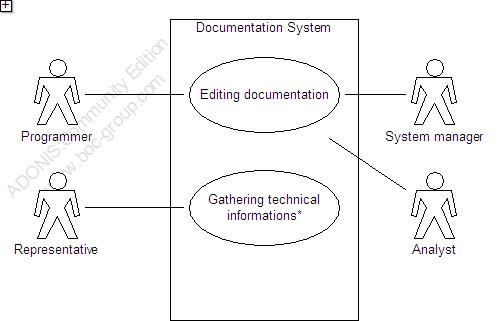
\includegraphics[scale=0.45]{assign3/adonis/imgs/documentation.jpg}
\caption{AllSpark Documentation management use case.}
\label{2img:[use]documentation}
\end{centering}
\end{figure}